\documentclass{vldb}
\usepackage{graphicx}
\usepackage[hyphens]{url}
\usepackage{balance}  % for  \balance command ON LAST PAGE  (only there!)


\newcommand{\eat}[1]{}
\newcommand{\red}{\textcolor{red}}
\newcommand{\system}{\textsc{Krypton}}

\vldbTitle{Demonstration of Krypton: Incremental and Approximate Inference for Faster Occlusion-based Deep CNN Explanations}
\vldbAuthors{Allen Ordookhanians et. al.}
\vldbDOI{https://doi.org/10.14778/xxxxxxx.xxxxxxx}
\vldbVolume{12}
\vldbNumber{xxx}
\vldbYear{2019}

\begin{document}

\title{Demonstration of Krypton: Incremental and Approximate Inference for Faster Occlusion-based Deep CNN Explanations}


\numberofauthors{1}
\author{
\alignauthor Allen Ordookhanians\hspace{10mm}Xin Li\hspace{10mm}Supun Nakandala\hspace{10mm}Arun Kumar\\
\affaddr{\vspace{2mm}University of California, San Diego}
\email{\{aordookh, xli222, snakanda, arunkk\}@eng.ucsd.edu}
}

\date{15 March 2019}


\maketitle

\begin{abstract}
In this demonstration we present \system, a system for accelerating occlusion based deep convolution neural network (CNN) explainability workloads.
Driven by the success of CNNs in image understanding tasks, there is growing adoption of CNN technology in various domains including high stake applications such as radiology.
However, users of such applications often seek an ``explanation'' for why a CNN predicted a certain label.
One of the widely used approaches for explaining the CNN predictions is the occlusion based explainability (OBE) method.
This approach is computationally expensive due to the large number of re-inference requests produced.
In this demo we present \system~, a system that reduces the runtime of OBE by up to 35x by enabling incremental and approximate inference optimizations.
We allow the audience to interactively diagnose CNN predictions from several use cases including radiology and natural images.
\end{abstract}




\section{Introduction}\label{introduction}
Deep Convolution Neural Networks (CNNs) are now the state of the art method for many image prediction tasks~\cite{imagenet}. Thus, there is growing interest in adopting deep CNNs in various application domains, including healthcare~\cite{kermany2018identifying, islam2017abnormality}, agriculture~\cite{mohanty2016using}, security~\cite{arbabzadah2016identifying}, and sociology~\cite{wang2017deep}. Remarkably, even the US Food and Drug Administration recently approved the use of deep CNNs in radiology to assist radiologists in processing X-rays and other scans, cross-checking their decisions, and even mitigating the shortage of radiologists~\cite{fdaretinopathy,radiologistshortage}.

Despite their successes, a key criticism of CNNs is that their internal workings are unintuitive to non-technical users. Thus, users often seek an ``explanation'' for why a CNN predicted a certain label. Explanations can help users trust CNNs~\cite{ribeiro2016should}, especially in high stakes applications such as radiology~\cite{jung2017deep}, and are a legal requirement for machine learning applications in some countries~\cite{gdpr}. How to explain a CNN prediction is still an active research question, but in the practical literature, an already popular mechanism for CNN explanations is a simple procedure called \textit{occlusion-based explanations}~\cite{zeiler2014visualizing}, or OBE for short.

OBE works as follows. Place a small square patch (usually gray) on the image to occlude those pixels. Rerun CNN inference, illustrated in Figure~\ref{fig:krypton_overview}(a), on the occluded image. The probability of the predicted class will change, as Figure~\ref{fig:krypton_overview}(b) shows. Repeat this process by moving the patch across the image to obtain a sensitivity \textit{heatmap} of probability changes, as Figure~\ref{fig:krypton_overview}(c) shows. This heatmap highlights regions of the image that were highly ``responsible'' for the prediction (red/orange color regions). Such localization of the regions of interest allows users to gain intuition on what ``mattered'' for the prediction. For instance, the heatmap can highlight the diseased areas of a tissue image, which a radiologist can then inspect more deeply for further tests. 
Overall, OBE is popular because it is easy for non-technical users to understand.

Alas, OBE is highly expensive computationally. Deep CNN inference is already expensive; OBE just amplifies it by issuing a large number of CNN re-inference requests (even 1000s). For example,~\cite{zintgraf2017visualizing} report 500,000 re-inference requests for 1 image, which took 1hr even on a GPU! Such long wait times can hinder users' ability to consume explanations and reduce their productivity. One could use more compute hardware, if available, since OBE is embarrassingly parallel across re-inference requests. But this may not always be affordable, especially for domain scientists, or feasible in all settings, e.g., in mobile clinical diagnosis. Extra hardware can also raise monetary costs, especially in the cloud.


\begin{figure*}[t]\label{img:ui}
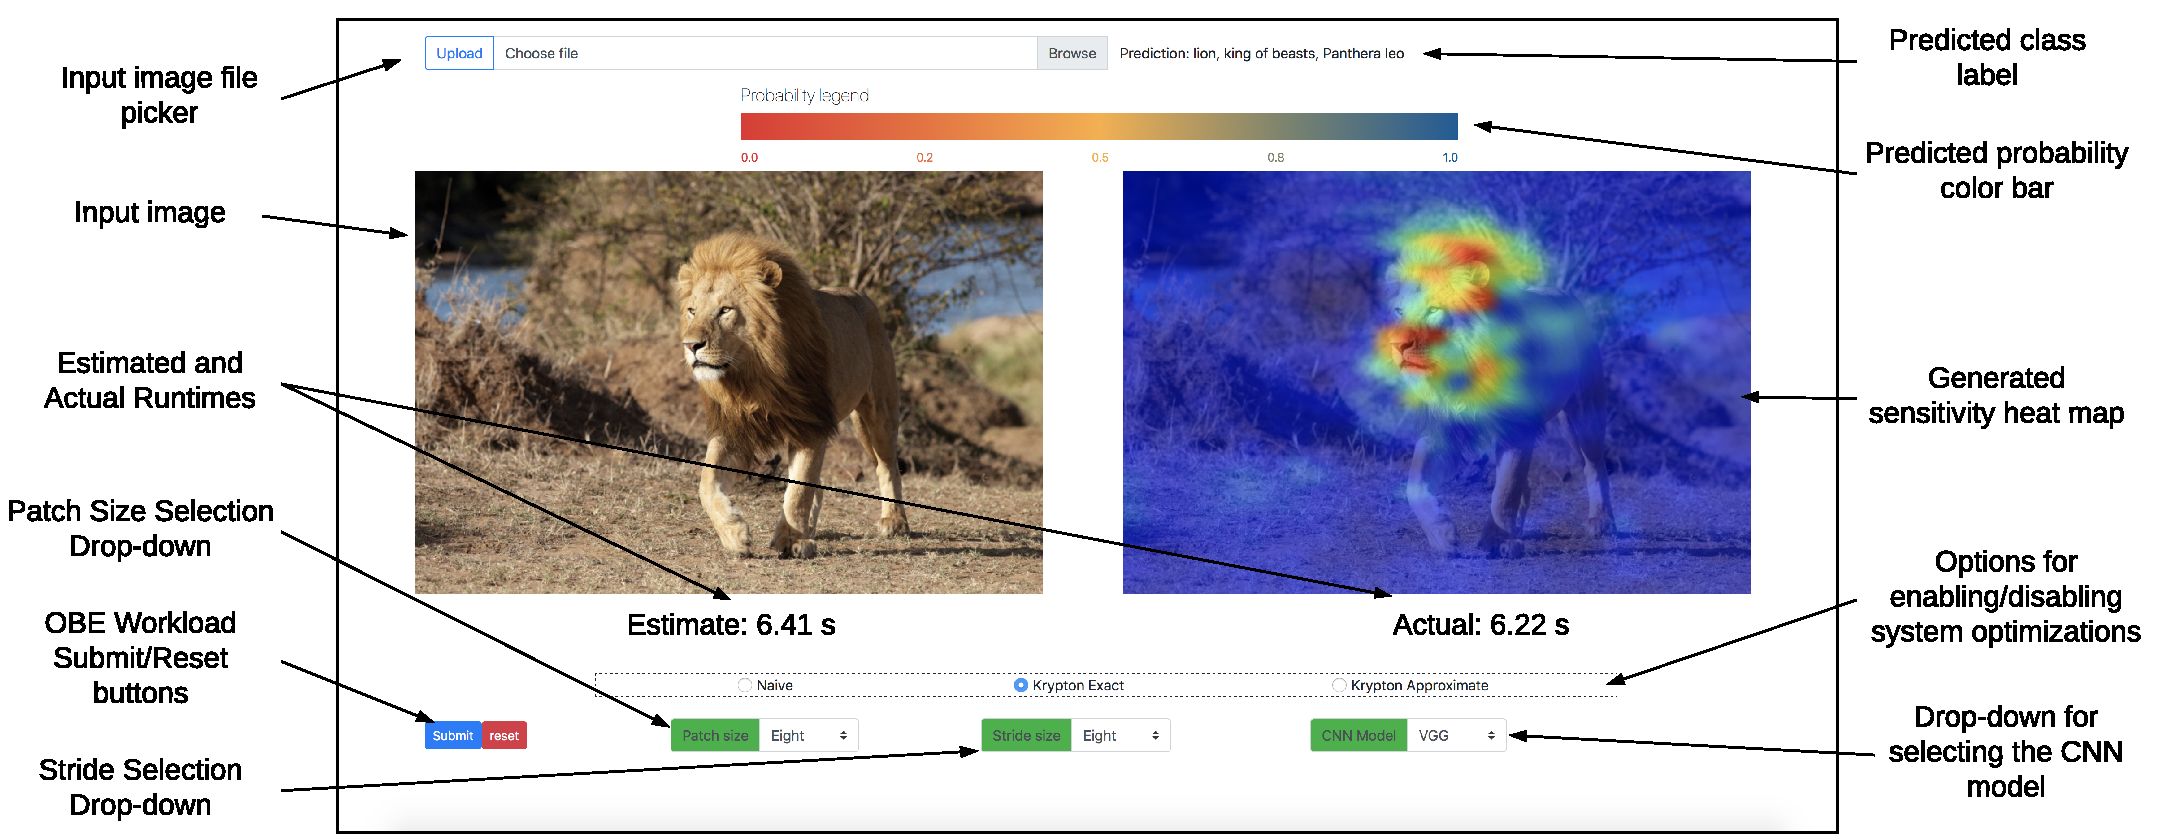
\includegraphics[width=\textwidth]{images/ui_actual.pdf}
\caption{\system~ user interface. Users can load an input image, select a CNN model and interactively diagnose the prediction by occluding parts of the full image or part of the image using the cropping tool. \system~ generates a sensitivity heat map (right image) and iteratively refines it as the user progresses.}
\end{figure*}

\system~ uses database-inspired lens to formalize, optimize, and accelerate OBE. We start with a simple but crucial observation: \textit{the occluded images are not disjoint but share most of their pixels; so, most of CNN re-inference computations are redundant.} This observation leads us to connect OBE with two classical data management concerns: \textit{incremental view maintenance} (IVM) and \textit{multi-query optimization} (MQO). Instead of treating a CNN as a ``blackbox,'' we open it up and formalize \textit{CNN layers} as ``queries.'' Just like how a relational query converts relations to other relations, a CNN layer converts \textit{tensors} (multidimensional arrays) to other tensors. So, we reimagine OBE as \textit{a set of tensor transformation queries} with incrementally updated inputs. With this fresh database-inspired view, we introduce several \textit{novel CNN-specific query optimization techniques} to accelerate OBE.

We prototype our ideas in the popular deep learning framework PyTorch to create a tool we call \system. It works on both CPU and GPU and currently supports a few popular deep CNNs (VGG16, ResNet18, and InceptionV3). We perform a comprehensive empirical evaluation of \system ~with three real-world image datasets from recent radiology and computer vision papers. \system ~yields up to $35$X speedups over the current dominant practice of running re-inference with just batching for producing high-quality approximate heatmaps and up to $5$X speedups for producing exact heatmaps.


\section{Technical Novelty}
The novelty of our system comes from the optimization techniques that it uses for accelerating the OBE workload.
In this section we briefly explain our \textit{incremental CNN inference} and \textit{approximate inference} optimizations.
More details on \system~ optimizations can be found in our Technical Report \cite{krypton}

\subsection{Incremental Inference}
With the incremental CNN inference optimization we \textit{materialize} all tensors produced by the CNN's layers on the given image. For every re-inference request in OBE, instead of rerunning CNN inference from scratch, we treat it as an incremental view maintenance (IVM) query, with the ``views'' being the tensors. We rewrite such queries to \textit{reuse} as much of the materialized views as possible and recompute only what is needed, thus \textit{avoiding computational redundancy}. Such rewrites are non-trivial because they are closely tied to the complex geometric dataflows of CNN layers. We have formalized such dataflows to create an \textit{algebraic framework} of CNN query rewrites. Going further, we batch all re-inference requests in OBE to reuse the \textit{same} materialized views. This is a form of multi-query optimization (MQO), albeit interwoven with our IVM, leading to a novel \textit{batched incremental CNN inference} procedure. To the best of our knowledge, this is the first instance of IVM being fused with MQO in query optimization, at least for CNN inference.

\begin{figure}
\includegraphics[width=\columnwidth]{images/redundancy_ratio.pdf}
\caption{Theoretical speedups for popular deep CNN architectures with incremental inference.}
\label{fig:theoretical_speedups}
\end{figure}

We calculate the max attainable theoretical speedup--in terms of the number computations saved--for performing IVM based incremental inference for popular CNN architectures with different occlusion patch sizes.
The results are shown in Figure \ref{fig:theoretical_speedups}.
VGG-16 has the highest theoretical speedups, while DenseNet-121 has the lowest. Most CNNs fall in the 2X–3X range.
The differences arise due to the specifics of the CNNs’ architectures: VGG-16 has small Convolution filter kernels and strides, which means full inference incurs a high computational cost (15 GFLOPs). In turn, incremental inference is most beneficial for VGG-16.
Note that we assumed an image size of 224$\times$224 for this plot; if the image is larger, the theoretical speedups will be higher.

While one might be tempted to think that speedups of 2X-3X may not be ``that significant'' in practice, we find that they indeed are significant for at least two reasons.
First, users often wait in the loop for OBE workloads for performing interactive diagnoses and analyses.
Thus, even such speedups can improve their productivity, e.g., reducing the time taken on a CPU from about 6min to just 2min, or on a GPU from
1min to just 20s.
Second, and equally importantly, incremental inference is the foundation for our approximate inference optimizations, which amplify the speedups we achieve for OBE.

\subsection{Approximate Inference}
The \textit{approximate inference} optimization in \system! allows users to tolerate some degradation in visual quality of the heat maps produced to reduce runtimes further.
This optimization build upon our incremental inference optimization to trade off heat map quality in a user-tunable manner.

We draws concept of \textit{projective field} from neuroscience and exploits the internal semantics of how CNNs work to reduce runtimes.
The projective field of a CNN neuron is the slice of the output tensor that is connected to it~\cite{basiccnnoperations}.
This notion sheds light on the \textit{growth of the size} of the update patches through the layers of a CNN.
Due to the overlapping nature of how convolution filter kernels operate the projective field of an updated patch in the input will grow after every layer.
It can be shown that in the projective field, the change in the pixels which are radially further aways from the center of the patch will be marginal.
To exploit this property we introduce the concept of \textit{projective field thresholding} which essentially truncates the growth of the projective field and save computations.

\begin{figure}[t]
\includegraphics[width=\columnwidth]{images/pf_truncate}
\caption{(a) Projective field growth for 1-D Convolution (filter size $2$, stride $1$). (b) Projective field \textit{thresholding}; $\tau = 5/7$.}
\label{fig:pf_truncate}
\end{figure}


To provide intuition on why the above happens, consider histograms on the side of Figures~\ref{fig:pf_truncate}(a,b) that list the number of unique ``paths'' from the updated element to each element in the last layer. It resembles a Gaussian distribution, with the maximum paths concentrated on the middle element. Thus, for most of the output patch updates, truncation will only discard a few values at the ``fringes'' that contribute to an output element. Of course, we do not consider the weights on these ``paths,'' which is dependent on the given trained CNN. Since the weights can be arbitrary, a tight formal analysis is unwieldy. But under some assumptions on the weights values (similar to the assumptions in~\cite{luo2016understanding} for understanding the ``receptive field'' in CNNs), it can be shown that this distribution does indeed converge to a Gaussian \cite{krypton}. Thus, while this idea is a heuristic, it is grounded in a common behavior of real CNNs.


\section{Demonstration}\label{demonstration}
\subsection{Datasets and CNN models.}
In this demonstration we will present an evaluation of \system ~with three real-world image datasets: 1) identifying diabetic retinopathy from retinal images, 2) identifying pneumonia from chest X-ray images, and 3) identifying objects from natural images in the ImageNet dataset.
\system~ currently supports three popular CNN architectures, VGG, ResNet, and Inception models. Altogether, each participant will be able to interact with the system on nine different settings.

\subsection{Walkthrough}
Each participant will be first made familiar with CNN models and OBE method in general.
This will be done using a supporting slide deck.
We will briefly cover important aspects such as different operators inside a CNN, the dataflow inside a CNN, and also the OBE approach for explaining CNN predictions.
This brief introduction will give the participants the necessary background to understand the \system~ system and appreciate its optimizations.
After the introduction participants will be demonstrated four scenarios of using \system.

\vspace{2mm}
\noindent \textbf{Scenario: Naive OBE.} In the first scenarios we will demonstrate performing OBE using the naive approach of performing CNN re-inference for each patch position.
Lets say we want to demonstrate the use of OBE to explain a prediction of an image from the ImageNet dataset from VGG16 model using a patch of size 8$\times$8 and a stride of 2.
We first loaf an image by clicking the file picker shown in Figure \ref{img:ui}.
After picking an image file, the image will be displayed on the left hand side panel of the interface.
Next we select the Naive option by clicking the corresponding radio button.
Selecting of the patch size, stride, and the CNN model can be also done using the corresponding drop-down menus as shown in Figure \ref{img:ui}.
We allow the user to pick from 4 different patch sizes (4$\times$4, 8$\times$8, 16$\times$16, 32$\times$32) and 4 different stride values (2, 4, 8, 16).
Current we support three different CNN model (VGG16, ResNet18, Inception3).

After picking the above values we can initiate OBE workload by clicking the submit button.
After submitting the workload, the system will display an estimate for the runtime of the workload as shown in Figure \ref{img:ui}.
This estimate is calculated using historical runtime statistics.
After the workload is completed the system will overlay an sensitivity heat map on the original image and display it on the right hand side panel.
On top of the heat map we show the predicted class label (e.g., lion) and also show the actual workload execution time.
On the heat map the red color regions corresponds to low predicted probabilities and the blue color regions correspond to high predicted probabilities. So the red color regions are the most sensitive regions for the predicted class label.
The color bar for the heat map is also shown in the interface.


\vspace{2mm}
\noindent \textbf{Scenario: \system~Exact.} After demonstrating the OBE workload using the naive approach we then demonstrate the utility of \system's incremental inference optimizations which we call \system~Exact.
Recall that incremental inference optimizations produce the exact same heat map produced by the naive approach but at a reduced computational cost.
\system~Exact scenarios is same as the previous scenario but with exception of picking the \system~Exact option from the radio button options instead of Naive option.
The estimated and actual runtimes for \system~Exact will be much smaller than Naive OBE.

\vspace{2mm}
\noindent \textbf{Scenario: \system~Approximate.} Next we will demonstrate the utility of \system's approximate inference optimizations which we call \system~Approximate.
Approximate inference optimizations trade-offs the accuracy of generated heat map with respect to the original heat map in favor of faster runtimes.
\system~Approximate scenarios is also same as the previous scenarios but with exception of picking the \system~Approximate option.
The estimated and actual runtimes for \system~Approximate will be even smaller than \system~Exact.
Though there will minor differences between the generated heat maps with \system~Exact and \system~Approximate the overall visual perception of both methods will very much similar.

\vspace{2mm}
\noindent \textbf{Scenario: Interactive Image Cropping.} So far in all of the above three cases we considered occlusion patch positions over the entire image.
However, this can be wasteful if the significant objects in an image are localized into a small region.
For example consider the image shown in Figure \ref{img:ui}.
The image contains an image of a lion on a wild background.
Clearly the main object in this image the lion which occupies only a small region of the entire image.
For a user who wants to diagnose the prediction for this image can start the diagnosis by selecting a smaller region which contains the face and the body of the lion by cropping that region.
If the user is not satisfied with the produced heat map he can iteratively refine the selected region.
The cropping of an image can be done simply by dragging on the image in the interface which selected rectangular selection areas.
Cropping operation is supported with all of the above three scenarios.

After going through the above four scenarios, participants will then be given the opportunity to use the system by them selves.
They will be able to select images from three different datasets: OCT images, Chest X-Ray images, and natural images from ImageNet dataset and will have the opportunity to \textit{interactively diagnose CNN predictions}.

\balance

\bibliographystyle{abbrv}
\bibliography{main}



\end{document}
